\newcommand\minilogo{
  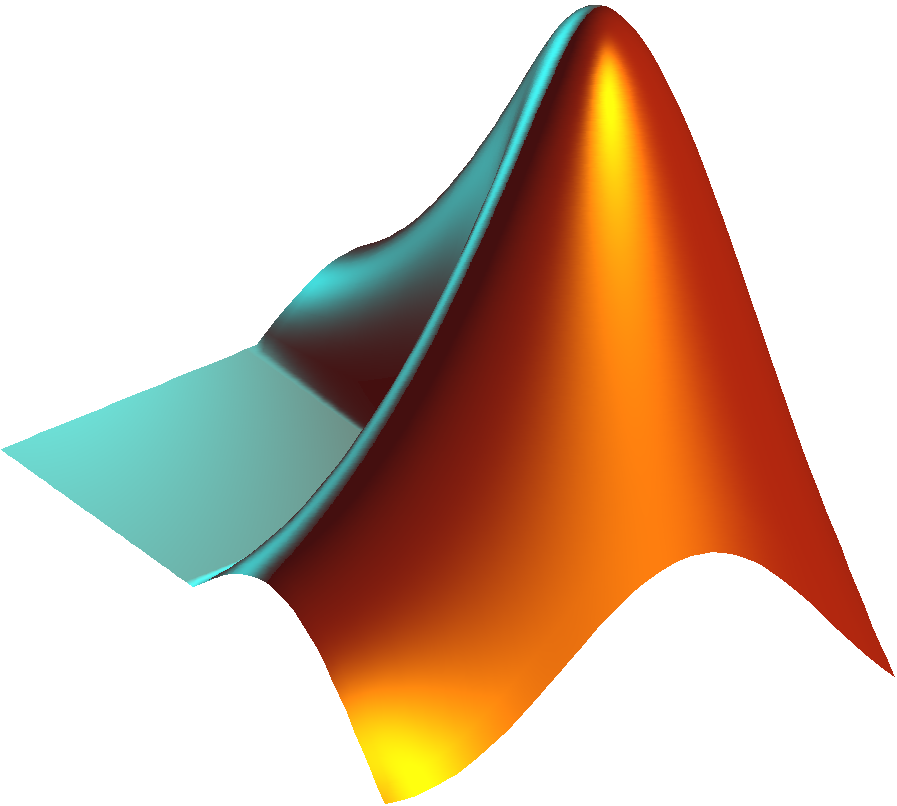
\includegraphics[width=0.5cm]{./media/Matlab_Logo.png}
}

\mode<article>{
En lo que sigue daremos una revisión
de los elementos de programación 
mínimos necesarios para esta materia.
Como lenguaje oficial elegimos 
\texttt{MATLAB}, no solo por razones
históricas, sino por su accesibilidad
para profesionales sin experiencia previa
en programación. En los casos donde sea posible, 
se darán las indicaciones equivalentes 
en otros lenguajes de uso corriente en la material 


% \begin{figure}
% \includeslide{FrameVentanaMatlab}
% \caption{Ventana de Matlab. se observan 
% el arbol de archivos del directorio
% de trabajo, el editor de guiones
% y la línea de comandos. 
% \label{FigMatlabInicio} }
% \end{figure}
}

\begin{frame}<presentation>[label=FrameMatlabPrimero]{Primeros Pasos en Matlab}
\begin{itemize}
\item[\minilogo] MATrix LABoratory
\item[\minilogo] Multiplataforma
\item[\minilogo] \url{http://www.mathworks.com/products/matlab}
\item[\minilogo] Lenguaje de programación, consola progrmable, ejecucion y redacción de scripts (guiones).
\end{itemize}
\end{frame}


\begin{frame}[label=FrameVentanaMatlab]
\frametitle<presentation>{Aspecto del Escritorio de Matlab}
%\mode<presentation>{
\begin{figure}
\begin{center}
\begin{tikzpicture}
\node [anchor=south west] (image) at (0,0) {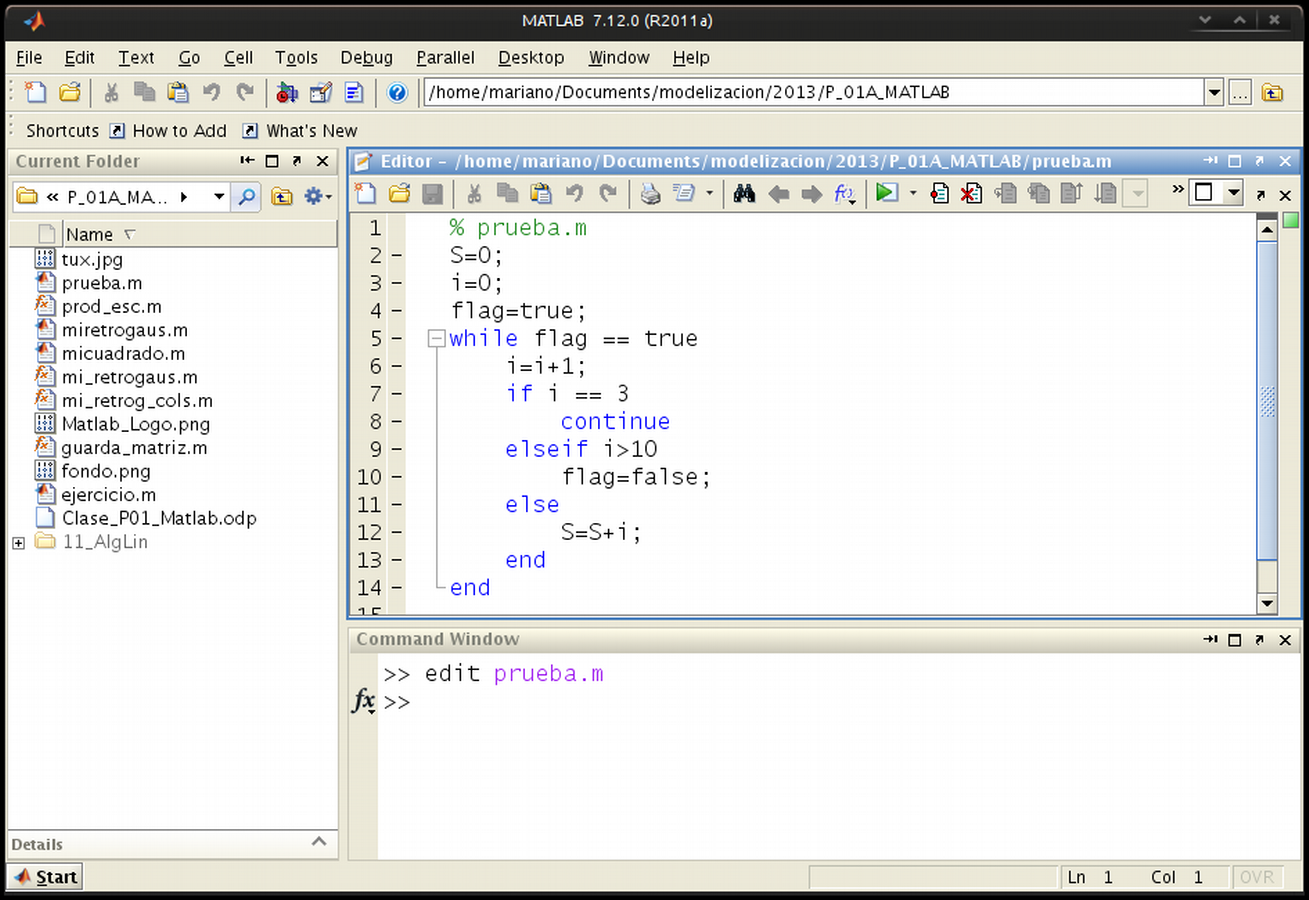
\includegraphics[width=0.7\textwidth]{./media/02-escritorio.png}};
\begin{scope}[x={(image.south east)},y={(image.north west)}]
  \node [rectangle,thick,fill=white,draw=black] at (0.15,0.2) {\small Archivos};
  \node [rectangle,thick,fill=white,draw=black] at (0.7,0.2) {\small  linea de comandos };
  \node [rectangle,thick,fill=white,draw=black] at (0.7,0.7) {\small  Editor de guiones };
\end{scope}
\end{tikzpicture}
\mode<article>{
 \caption{Ventana de Matlab. se observan 
 el arbol de archivos del directorio
 de trabajo, el editor de guiones
 y la línea de comandos. 
 \label{FigMatlabInicio}
  }
}
\end{center}
\end{figure}
%}
\mode<article>{
Busque en su pc el ícono de inicio de MATLAB, o bien inicie el programa
desde la línea de comandos. 

 Al inicar MATLAB en cualquier plataforma, se observan las ventanas de la 
 \autoref{FigMatlabInicio}. Revise las configuraciones para obtener
el escritorio que le sea cómodo. Sin embargo, puede encontrar de 
 utilidad un escritorio como el que se muestra. 

 Si bien especificamos las indicaciones para esta herramienta 
 en particular, la estructura general vale para cualquier 
 Entorno Integrado de Desarrollo (IDE) que pueda encontrar. 
} 
\end{frame}
